% Chapter 3 — Human Resources. Authorized draft, submitted for review after the build.
\chapter{Human Resources}
\label{ch:hr}

\section{What you will achieve}

\textbf{Result:} know who works, their working time, and how to review leave and pay. Start with Sarah, then repeat for the team.

\section{HR pages at a glance}

Start with people and structure, then time, then payroll if used. This is priority order; prepare units and locations before linking positions. Sections vary by setup and permissions; search by page name.

\textbf{Open:} HR / listed section / page. Setup walkthrough: Section~\ref{sec:setup-data}.

\begin{figure}[H]
\centering
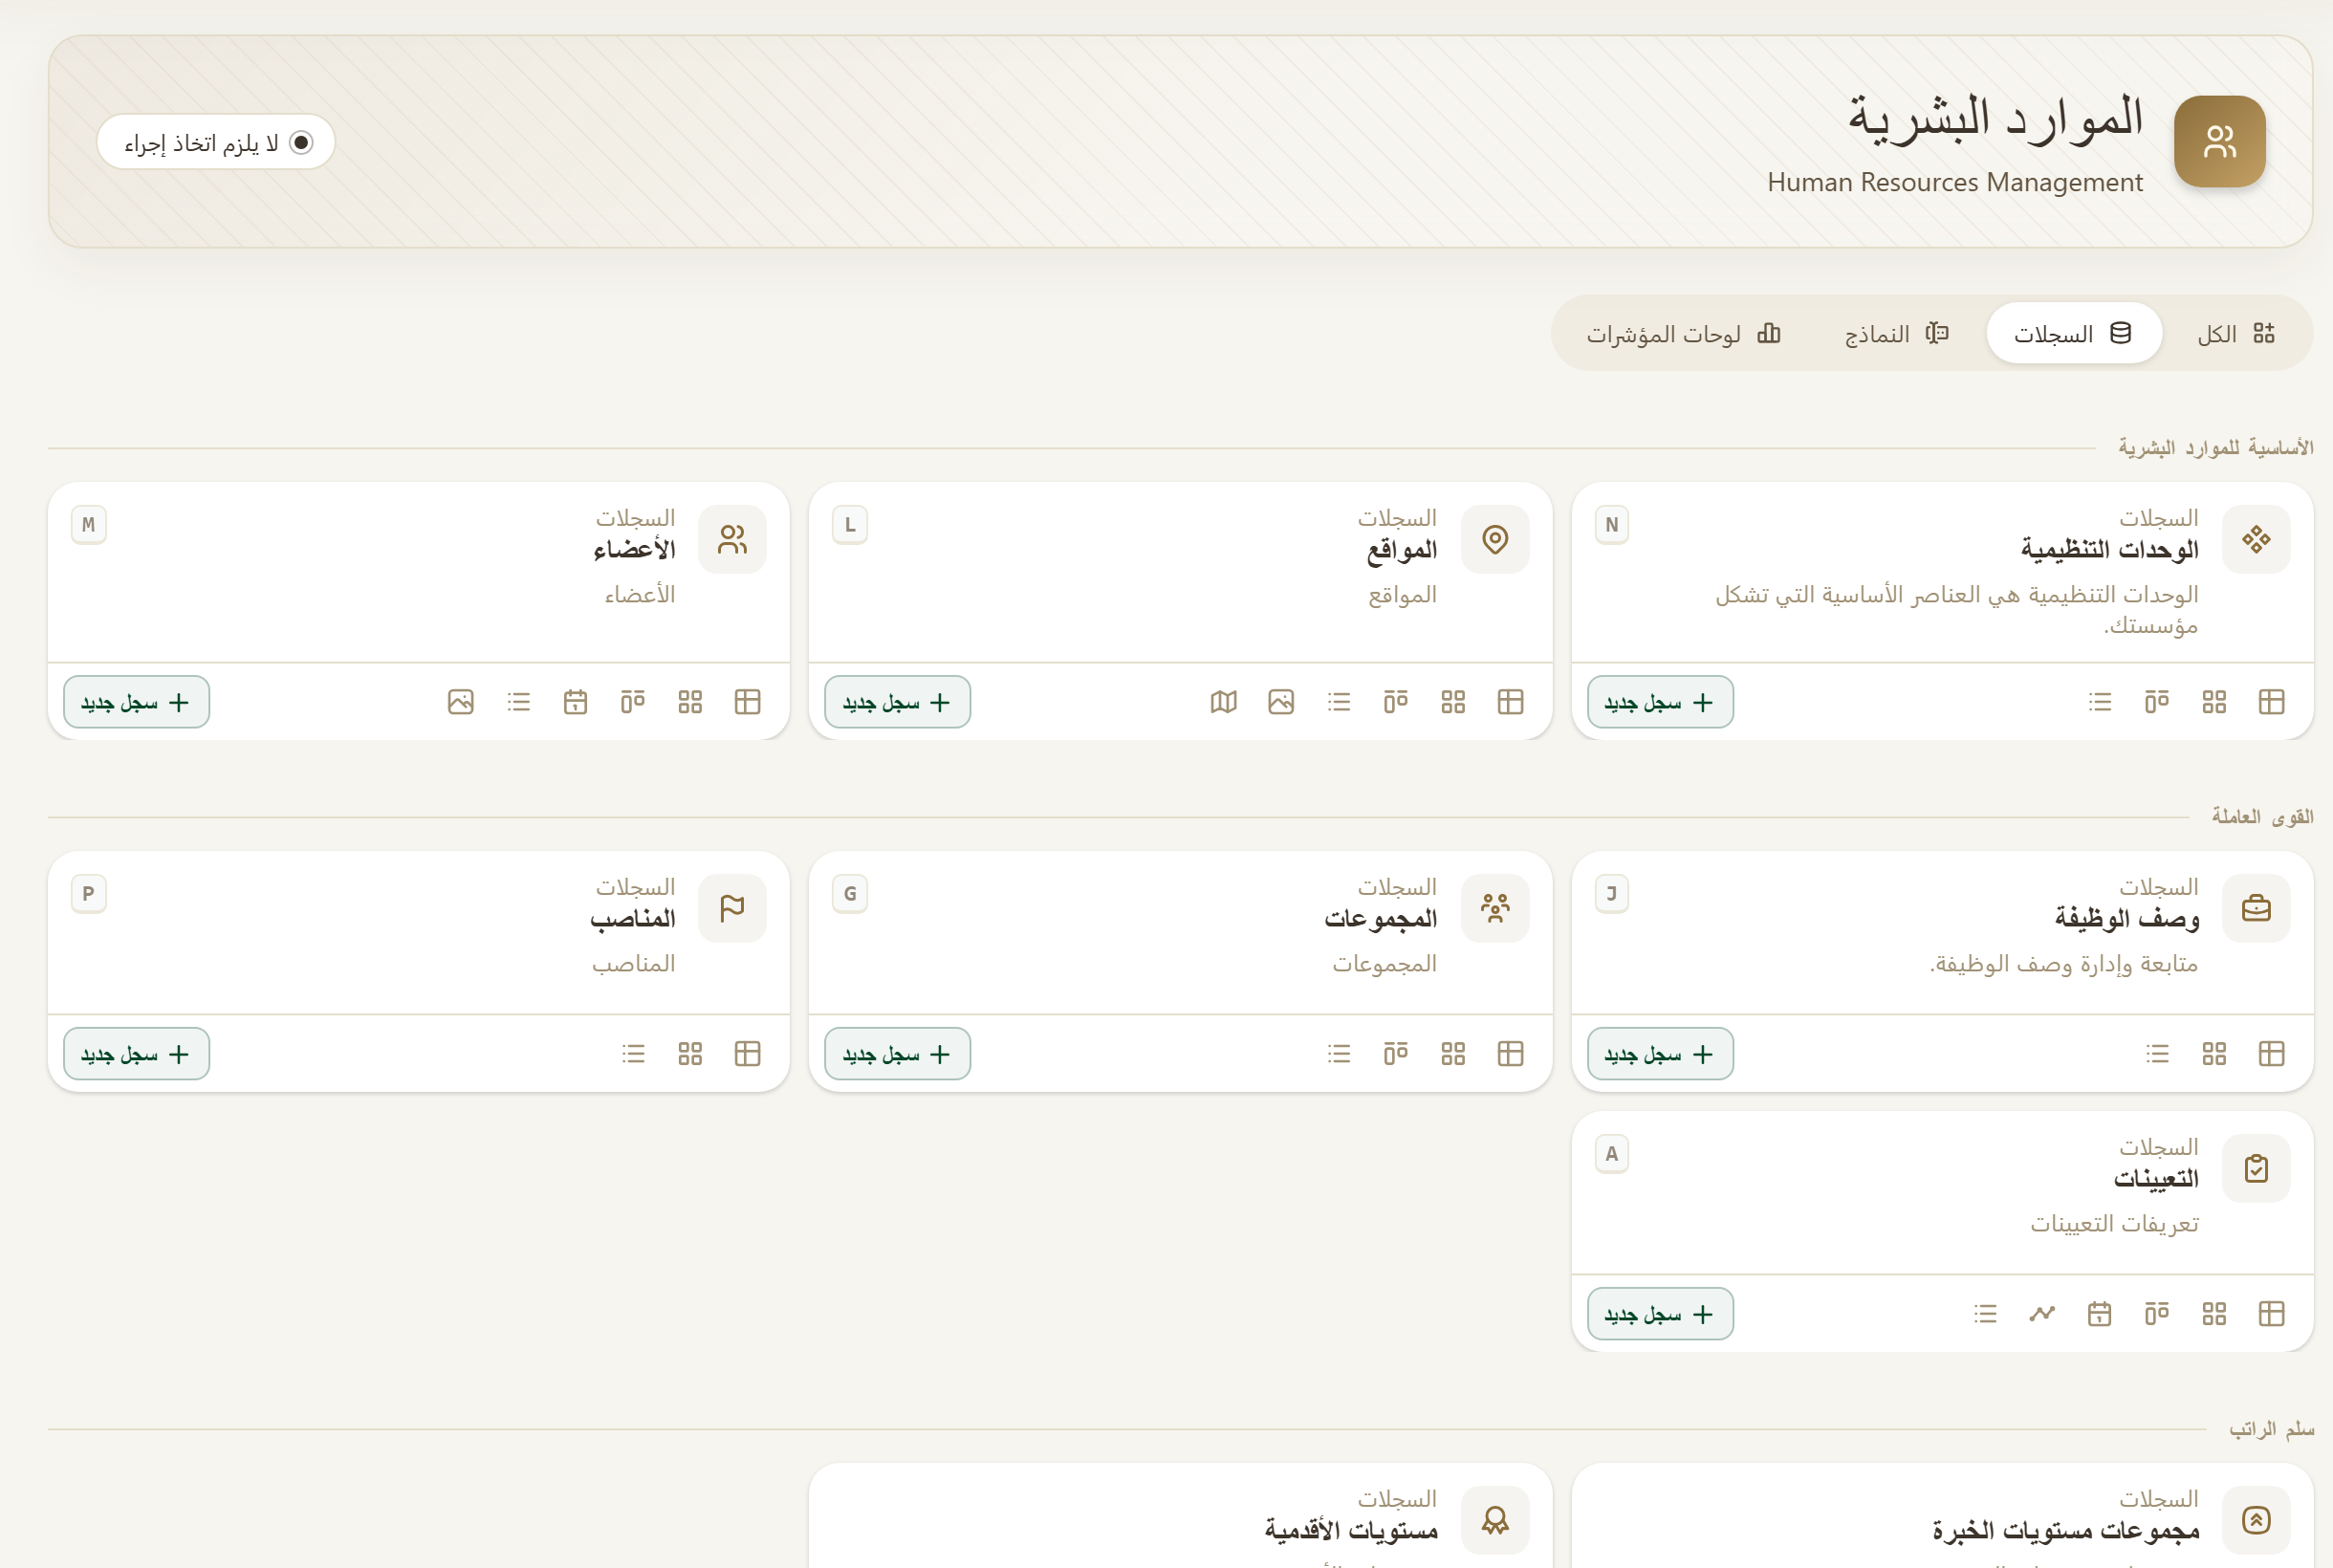
\includegraphics[width=0.95\linewidth]{figures/screens/ch03-hr-pages-clear.png}
\caption{Structure and people pages (Arabic interface)}
\label{fig:hr-pages-screen}
\end{figure}

\begin{table}[H]
\centering
\caption{People and structure: first priority}
\label{tab:hr-pages-core}
\rcZebra
\begin{tabularx}{\linewidth}{R{4.2cm} Y}
\rcHeaderRow
\thh{Page and section} & \thh{What this page offers}\\
Members — Workforce & Add and update employee records and personal details.\\
Positions — Workforce & Define jobs and link them to departments and work locations.\\
Assignments — Workforce & Link each employee to a job for a defined period, with an assignment status.\\
Nodes — Core & Organize departments and divisions into a hierarchy.\\
Locations — Core & Manage work sites, their addresses and their location hierarchy.\\
Groups — Workforce & Bring members together into teams without changing their job assignments.\\
\end{tabularx}
\end{table}

\begin{table}[H]
\centering
\caption{Following the working day: Time pages}
\label{tab:hr-pages-time}
\rcZebra
\begin{tabularx}{\linewidth}{R{4.2cm} Y}
\rcHeaderRow
\thh{Page and section} & \thh{What this page offers}\\
Shifts — Time & Set working days, hours and breaks for each schedule.\\
My attendance — Time & View your daily attendance, clock-in and clock-out times, and worked duration.\\
Timesheets — Time & Review recorded working time across employees and date ranges.\\
Leave Types — Time & Define reusable leave types and how each affects pay.\\
Leaves — Time & Record employee leave with its type, dates, duration and status.\\
Holiday Groups — Time & Organize shared holidays and link them to the relevant units or jobs.\\
Attendance Corrections — Time & Submit attendance correction requests and track their review status.\\
Attendance policy — Time & Set the rules used to evaluate attendance, such as lateness and overtime.\\
Attendance terminals — Time & Manage attendance devices and match their records to employees.\\
\end{tabularx}
\end{table}

\begin{table}[H]
\centering
\caption{When running payroll: setup, then review}
\label{tab:hr-pages-pay}
\rcZebra
\begin{tabularx}{\linewidth}{R{4.2cm} Y}
\rcHeaderRow
\thh{Page and section} & \thh{What this page offers}\\
Seniority Levels — Salary Scale & Define the job grades used in the salary scale.\\
Experience Levels — Salary Scale & Organize experience levels and their values within experience groups.\\
Salary Scale — Salary Scale & View and set salary values at the intersection of job and experience levels.\\
Payroll Inputs — Payment & Record variable pay items for a period and preview their calculation.\\
Salary Slips — Payment & Calculate and review each employee’s earnings, deductions and net pay.\\
Payrolls — Payment & Group approved salary slips into a payroll and review its totals and status.\\
\end{tabularx}
\end{table}

Experience levels and holiday dates are inside their groups, not extra app pages.

\begin{figure}[H]
\centering
\begin{tikzpicture}[node distance=0.7cm]
  \node[entity] (asg) {Assignments};
  \node[entity,below right=0.7cm and 0.5cm of asg] (mem) {Members};
  \node[entity,below left=0.7cm and 0.5cm of asg] (pos) {Positions};
  \node[entityOpt,below right=0.7cm and 0.1cm of pos] (node) {Nodes};
  \node[entityOpt,below left=0.7cm and 0.1cm of pos] (loc) {Locations};
  \draw[dependsOn] (asg.south) -- ++(0,-0.3) -| (mem.north);
  \draw[dependsOn] (asg.south) -- ++(0,-0.3) -| (pos.north);
  \draw[dependsOnOpt] (pos.south) -- ++(0,-0.3) -| (node.north);
  \draw[dependsOnOpt] (pos.south) -- ++(0,-0.3) -| (loc.north);
\end{tikzpicture}
\rclegend
\caption{Assignment links person and job}
\label{fig:hr-models}
\end{figure}

Read from the assignment to the records it needs. Sarah is the member; HR Manager is the position. Unit and location links are optional. Groups do not replace these links.

\begin{figure}[H]
\centering
\begin{tikzpicture}[node distance=0.4cm,stepBox/.append style={minimum width=6.5cm,text width=6.1cm,minimum height=0.7cm}]
  \node[stepBox] (m0) {Assignment and\\employee data};
  \node[stepBox,below=of m0] (m1) {Review time and leaves};
  \node[stepBox,below=of m1] (m2) {Review payroll inputs};
  \node[stepBox,below=of m2] (m3) {Calculate and approve\\salary slip};
  \node[stepBox,below=of m3] (m4) {Generate and review\\payroll};
  \draw[flowsTo] (m0) -- (m1);
  \draw[flowsTo] (m1) -- (m2);
  \draw[flowsTo] (m2) -- (m3);
  \draw[flowsTo] (m3) -- (m4);
\end{tikzpicture}
\rclegend
\caption{Review path from the employee to payroll}
\label{fig:hr-review-flow}
\end{figure}

Dashed arrows are review steps, not automatic processing. Skip payroll if you only need to organize the team.

\section{Check the assignment}

Open HR / Workforce / Assignments. Check Sarah’s member, position and start date. If missing, follow Section~\ref{sec:setup-data}. Keep the same member record when her job changes.

\section{Create a shift}
\label{sec:hr-shifts}

A shift sets expected time; attendance shows what happened. Owner: HR.

\begin{table}[H]
\centering
\caption{Choosing the shift type}
\label{tab:hr-shift-types}
\rcZebra
\begin{tabularx}{\linewidth}{R{2.4cm} Y Y}
\rcHeaderRow
\thh{Type} & \thh{What do you enter?} & \thh{Example}\\
Regular & A set work period, with a break when needed. & From 09:00 to 17:00.\\
Split & More than one work period, without overlap. & From 09:00 to 13:00, then from 16:00 to 20:00.\\
Flexible & The required work duration in hours and minutes. & A duration of 08:00; no start and end period is set in the form.\\
Marathon & The required work duration, as the form shows it for this type. & The guide does not assume an automatic cycle of work and rest days from the name alone.\\
\end{tabularx}
\end{table}

\begin{enumerate}
  \item HR / Time / Shifts: add “Office Hours”, code HZN-S-01, type “Regular”.
  \item Choose Sunday–Thursday and Asia/Damascus. Name, code, type and at least one workday are \req{}.
  \item Work Hours: 09:00–17:00. Edit the existing break to 13:00–13:30; do not add a duplicate. Breaks are \opt{}.
  \item Check Total Hours = 07:30, then “Save”. Reopen and check the values.
\end{enumerate}

\begin{figure}[H]
\centering
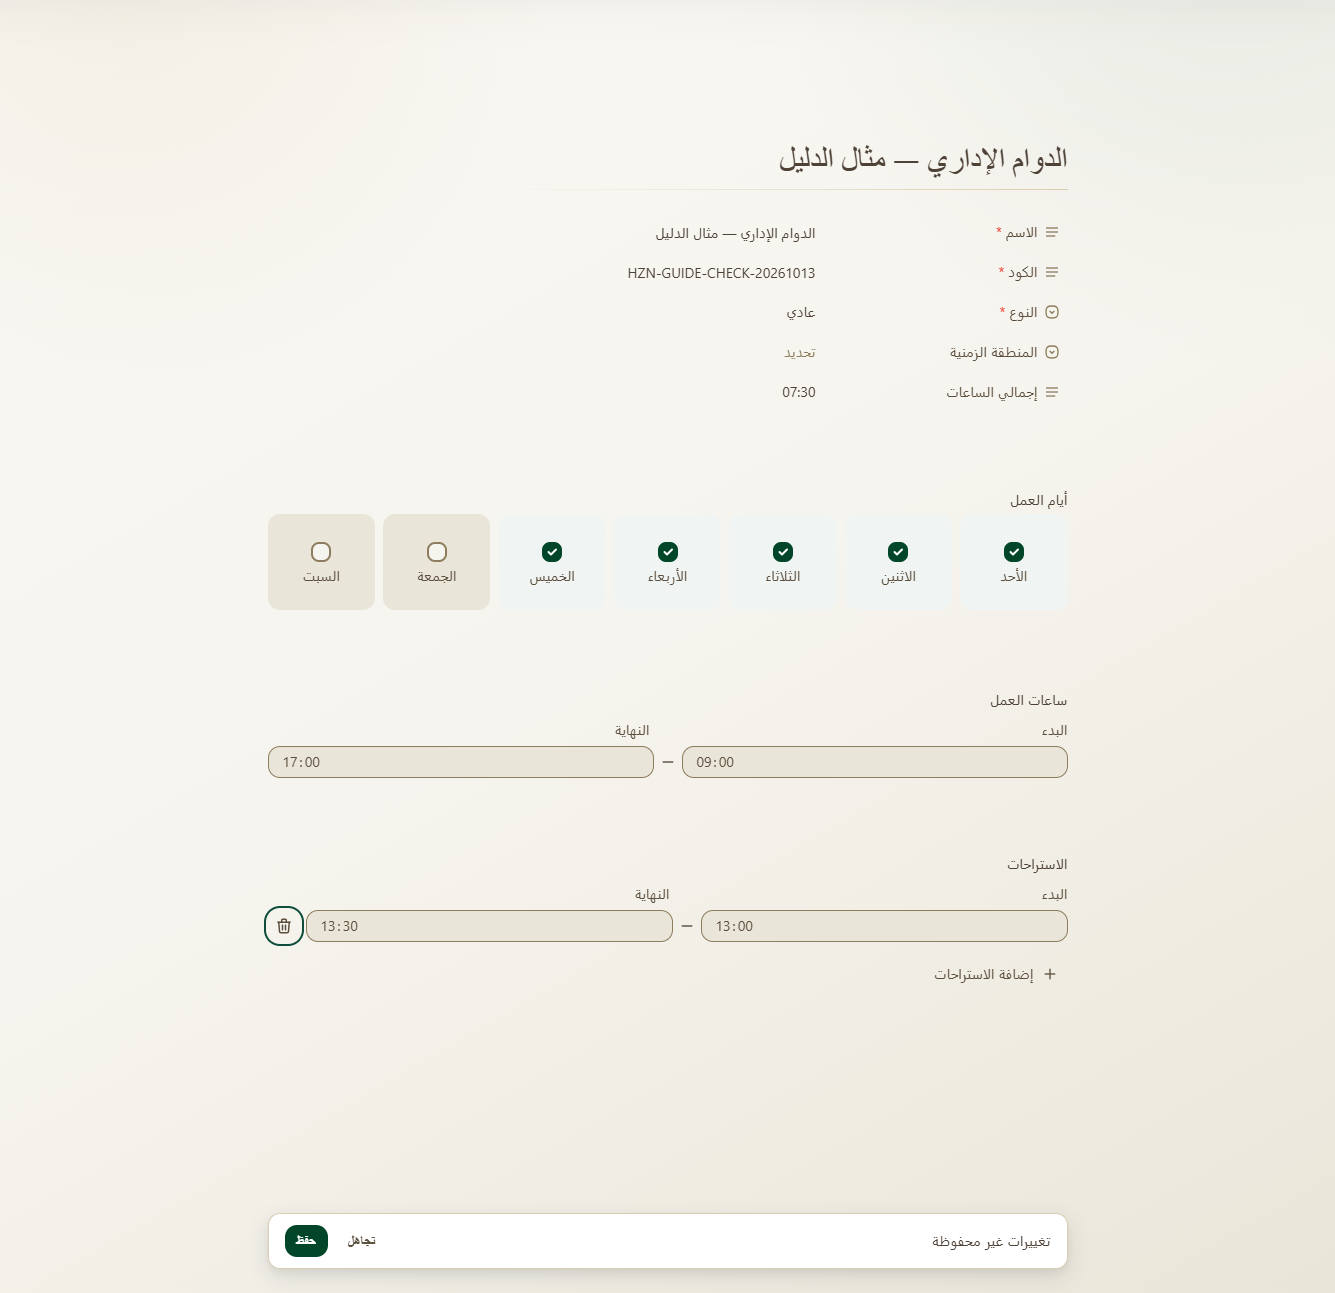
\includegraphics[width=0.9\linewidth]{figures/screens/ch03-shift-example.png}
\caption{Unsaved Arabic test form: five days, a half-hour break, total 07:30}
\label{fig:hr-shift-screen}
\end{figure}

The image demonstrates hours; use the code and timezone in the steps above. For split shifts, add each period. For flexible/marathon shifts, enter hours and minutes.

\begin{rcnote}[Avoid time errors]
Periods must not overlap; breaks stay inside work time. 22:00–06:00 ends the next day. Equal start/end does not mean a full day.
\end{rcnote}

When importing, check the preview; template and form fields differ by type.

\section{How the shift reaches the employee}
\label{sec:hr-shift-inheritance}

Inheritance: use a shift from a higher record instead of repeating it.

\begin{figure}[H]
\centering
\begin{tikzpicture}[node distance=0.4cm,stepBox/.append style={minimum width=6.5cm,text width=6.1cm,minimum height=0.7cm}]
  \node[stepBox] (a) {Assignment shift};
  \node[stepBox,below=of a] (p) {Position shift};
  \node[stepBox,below=of p] (n) {Unit shift, then its\\parent units};
  \node[stepBox,below=of n] (l) {Location shift, then\\its parent locations};
  \draw[flowsTo] (a) -- (p);
  \draw[flowsTo] (p) -- (n);
  \draw[flowsTo] (n) -- (l);
\end{tikzpicture}
\rclegend
\caption{Order of the shift search: move to the next level only if no shift is found}
\label{fig:hr-shift-order}
\end{figure}

Stop at the first shift found. Unit and parents precede location and parents; shifts are not combined.

\begin{enumerate}
  \item Open HR / Core / Nodes / HZN-HR.
  \item Select “Office Hours” in “Shift”. Use “Override” if needed to choose it, then save.
  \item Open Workforce / Positions / HR Manager. Check unit and shift.
  \item Open Sarah’s assignment and check the shift. If different, check assignment then position as shown.
\end{enumerate}

“Reset” restores inheritance. After changing a unit’s shift, check assignments with overrides.

\section{Review an attendance day}
\label{sec:hr-time}

You need an assignment, shift and recorded attendance. Creating an employee does not create past attendance.

\begin{figure}[H]
\centering
\begin{tikzpicture}[node distance=0.4cm,stepBox/.append style={minimum width=6cm,text width=5.6cm,minimum height=0.7cm}]
  \node[stepBox] (s0) {My attendance: month\\and day};
  \node[stepBox,below=of s0] (s1) {Compare shift and\\clocking times};
  \node[stepBox,below=of s1] (s2) {Check any leave or\\holiday};
  \node[stepBox,below=of s2] (s3) {Check correction and\\decision};
  \draw[flowsTo] (s0) -- (s1);
  \draw[flowsTo] (s1) -- (s2);
  \draw[flowsTo] (s2) -- (s3);
\end{tikzpicture}
\rclegend
\caption{Review one day}
\label{fig:hr-day-review}
\end{figure}

\begin{enumerate}
  \item Open HR / Time / My attendance, then month and day. Viewing another member requires permission.
  \item Compare shift, clocking times and duration. For a period or several employees, open “Timesheets” and set people and dates.
  \item For a discrepancy, check the source with the attendance administrator. Open “Attendance Corrections” for an available correction; check member, date and decision.
\end{enumerate}

\textbf{Check:} you can explain the difference. If empty, check member, period, permission and source; an empty screen does not prove absence.

\begin{rcnote}[Shift and policy]
The shift sets expected time; policy handles lateness and overtime. Review the result; do not assume automatic deductions or pay.
\end{rcnote}

\section{Holidays and leave}

A holiday is shared; leave belongs to an employee. A leave type is a reusable rule; a leave record applies it on a date.

\begin{figure}[H]
\centering
\begin{tikzpicture}[node distance=0.4cm,stepBox/.append style={minimum width=6cm,text width=5.6cm,minimum height=0.7cm}]
  \node[stepBox] (s0) {Review type and\\payment};
  \node[stepBox,below=of s0] (s1) {Obtain required\\approval};
  \node[stepBox,below=of s1] (s2) {Record employee, date\\and duration};
  \node[stepBox,below=of s2] (s3) {Save; review the day\\and pay};
  \draw[flowsTo] (s0) -- (s1);
  \draw[flowsTo] (s1) -- (s2);
  \draw[flowsTo] (s2) -- (s3);
\end{tikzpicture}
\rclegend
\caption{From leave type to reviewing the employee’s day}
\label{fig:hr-leave-flow}
\end{figure}

This is a workflow, not automatic approval. Owner: HR.

\begin{enumerate}
  \item HR / Time / Leave Types: search first. If a new type is needed and permitted, add “Annual (paid)”, choose payment treatment and the percentage for partial pay. Save and check.
  \item Check that the type is available in the employee’s job settings; its existence does not grant entitlement to everyone.
  \item After approval: Time / Leaves / add. Select Sarah, type, start/end times and the authorized status. Duration is calculated. Save.
  \item Reopen and check person, type, date and duration. Review the period in attendance and pay.
\end{enumerate}

\begin{figure}[H]
\centering
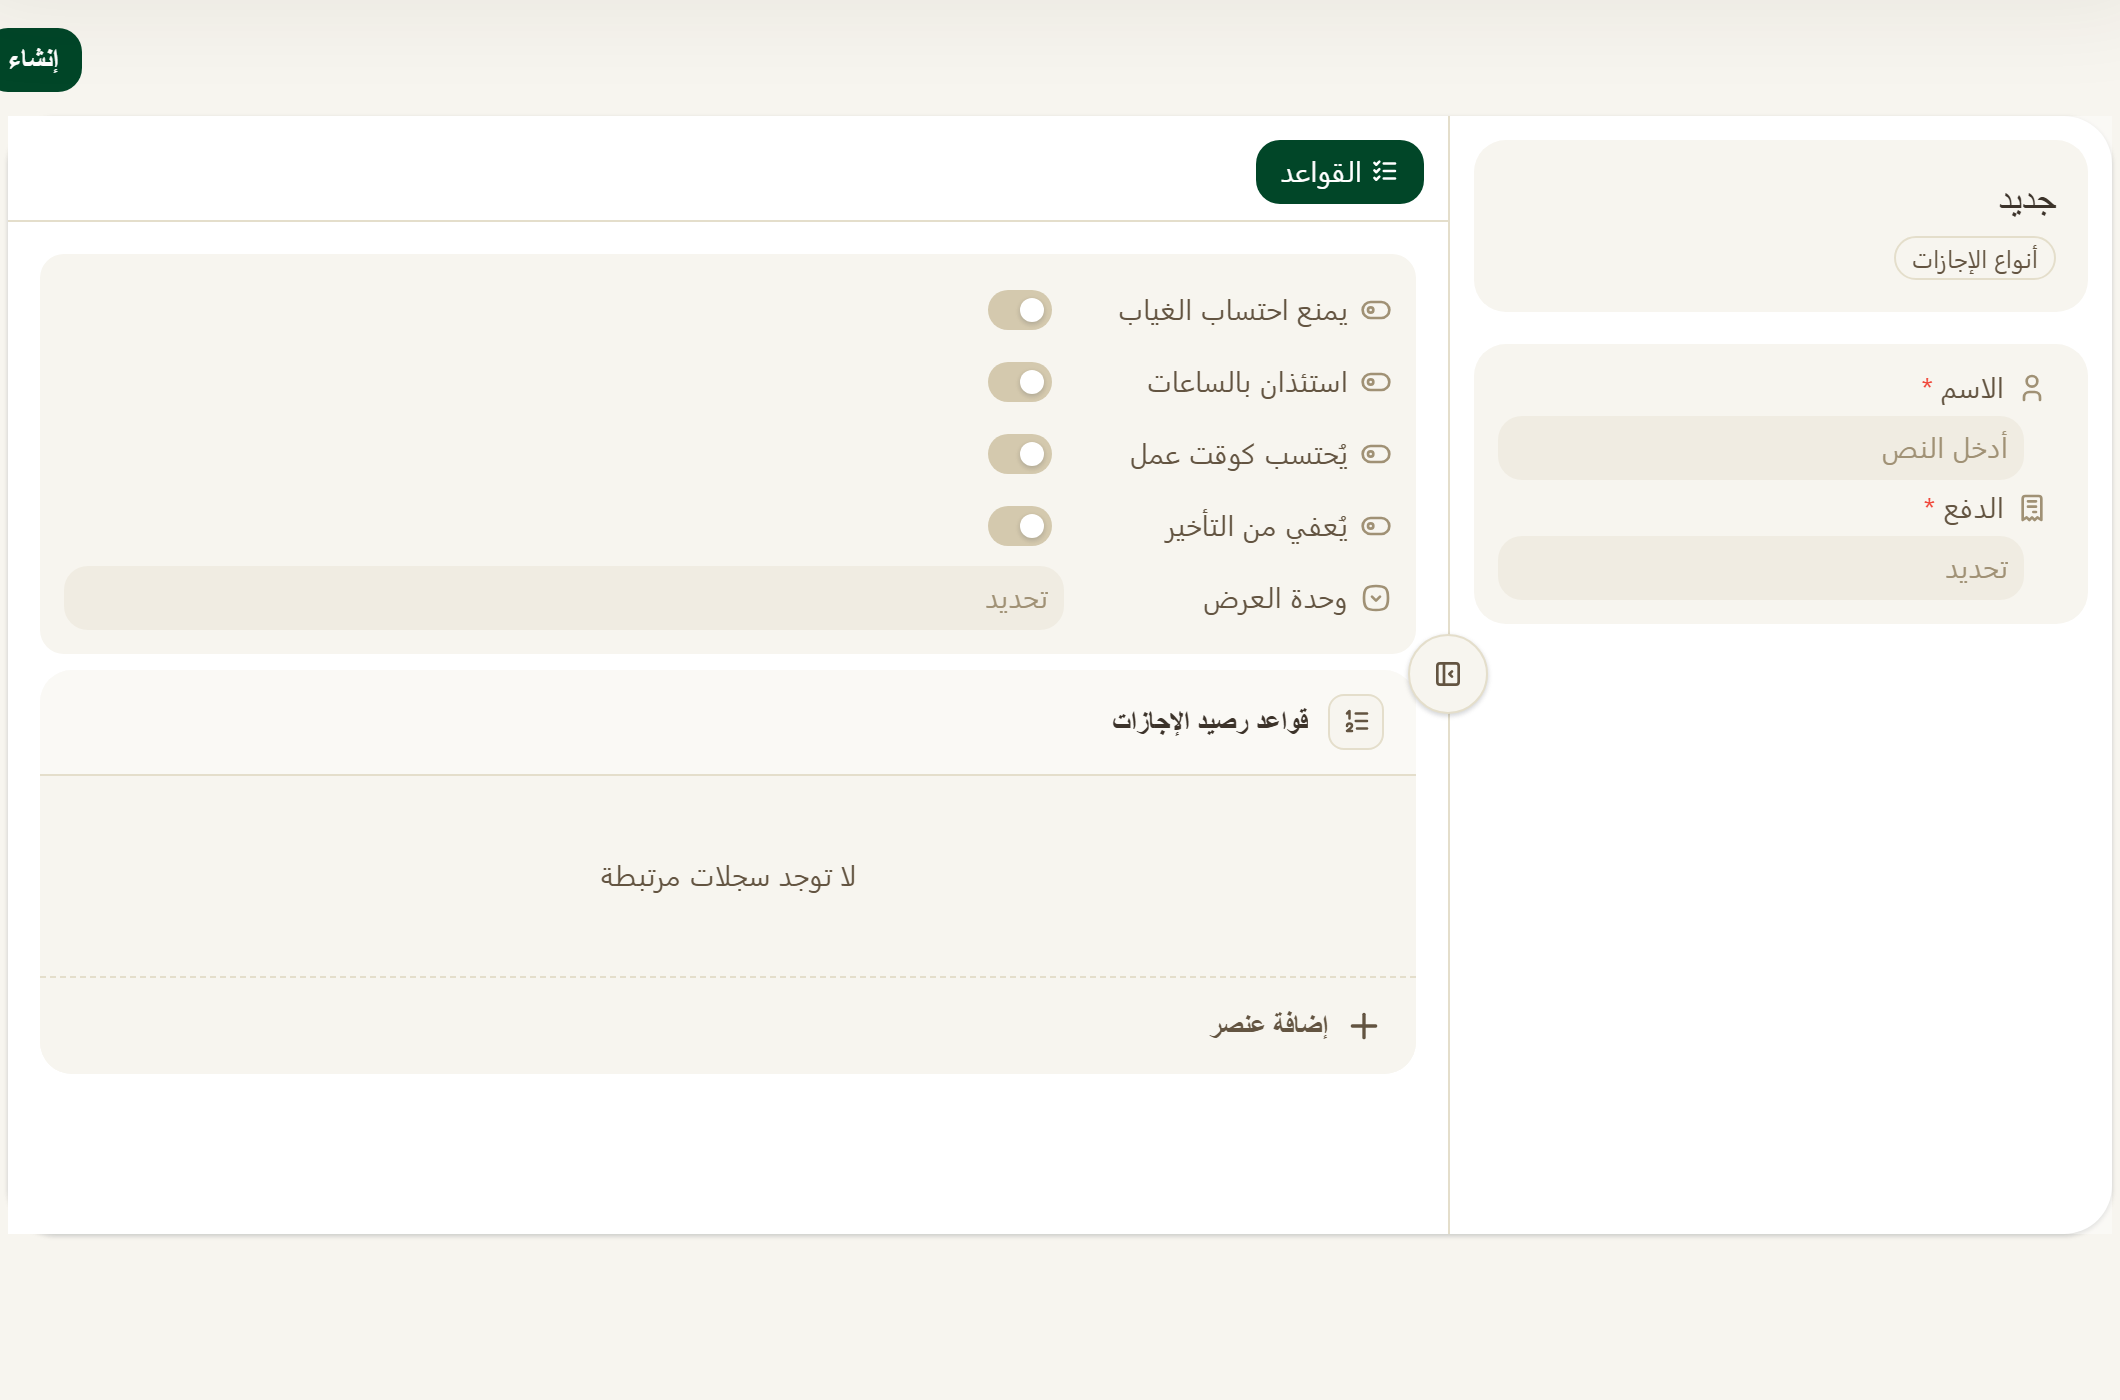
\includegraphics[width=0.95\linewidth]{figures/screens/ch03-leave-type-fields.png}
\caption{Leave type: payment and rules — unsaved Arabic form}
\label{fig:hr-leave-type-screen}
\end{figure}

\begin{figure}[H]
\centering
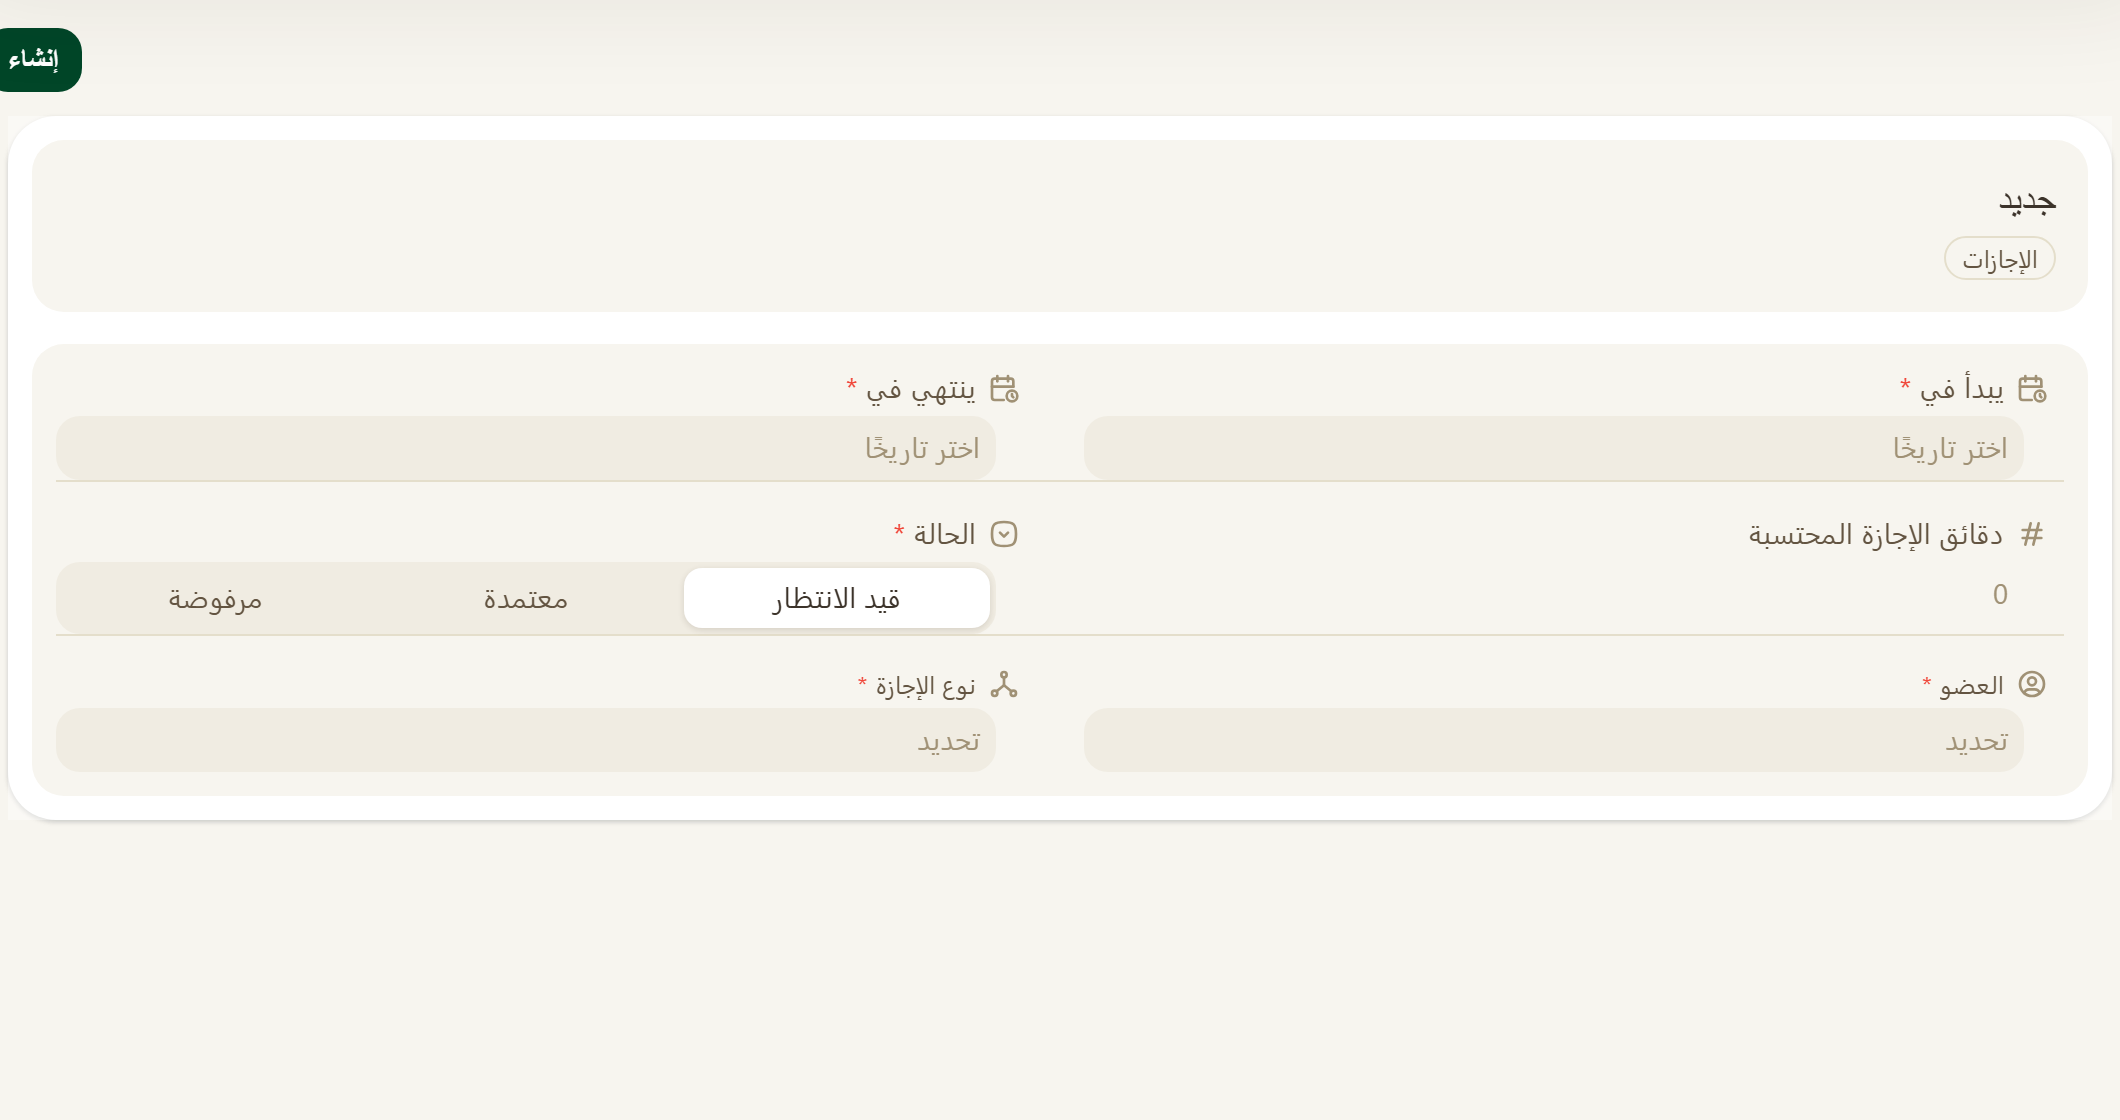
\includegraphics[width=0.95\linewidth]{figures/screens/ch03-leave-fields.png}
\caption{Leave: employee, dates and status — unsaved Arabic form}
\label{fig:hr-leave-screen}
\end{figure}

\textbf{Shared holidays:} Time / Holiday Groups / group. Add name, date and full day, partial day or period. Enter partial-day hours or period start/end; save and check links to units or jobs.

\textbf{If the effect is missing:} check date, type, links and status. Submitting a request does not mean leave is approved and recorded.

\section{Prepare pay data}
\label{sec:hr-payroll}

Owner: payroll staff after time review. The salary scale is a reference; assignment data is still needed.

\begin{figure}[H]
\centering
\begin{tikzpicture}[node distance=0.4cm,stepBox/.append style={minimum width=6cm,text width=5.6cm,minimum height=0.7cm}]
  \node[stepBox] (s0) {Experience: group and\\increases};
  \node[stepBox,below=of s0] (s1) {Seniority levels: pay\\values};
  \node[stepBox,below=of s1] (s2) {Salary Scale: check\\intersections};
  \node[stepBox,below=of s2] (s3) {Assignment: check pay\\and currency};
  \draw[flowsTo] (s0) -- (s1);
  \draw[flowsTo] (s1) -- (s2);
  \draw[flowsTo] (s2) -- (s3);
\end{tikzpicture}
\rclegend
\caption{If your organization uses a salary scale}
\label{fig:hr-scale-setup}
\end{figure}

In Salary Scale, save the experience group, levels, increase rule and currency, then seniority levels and values. Open the matrix and check intersections. Arrows show setup order, not automatic payment.

\begin{enumerate}
  \item Check assignment period, pay, currency, time, leave and corrections.
  \item HR / Payment / Payroll Inputs: search first to avoid duplicates.
  \item To add: complete * fields, the period and approved amount. Save and open “Preview calculation”. Correct discrepancies, then complete authorized approval.
\end{enumerate}

\begin{figure}[H]
\centering
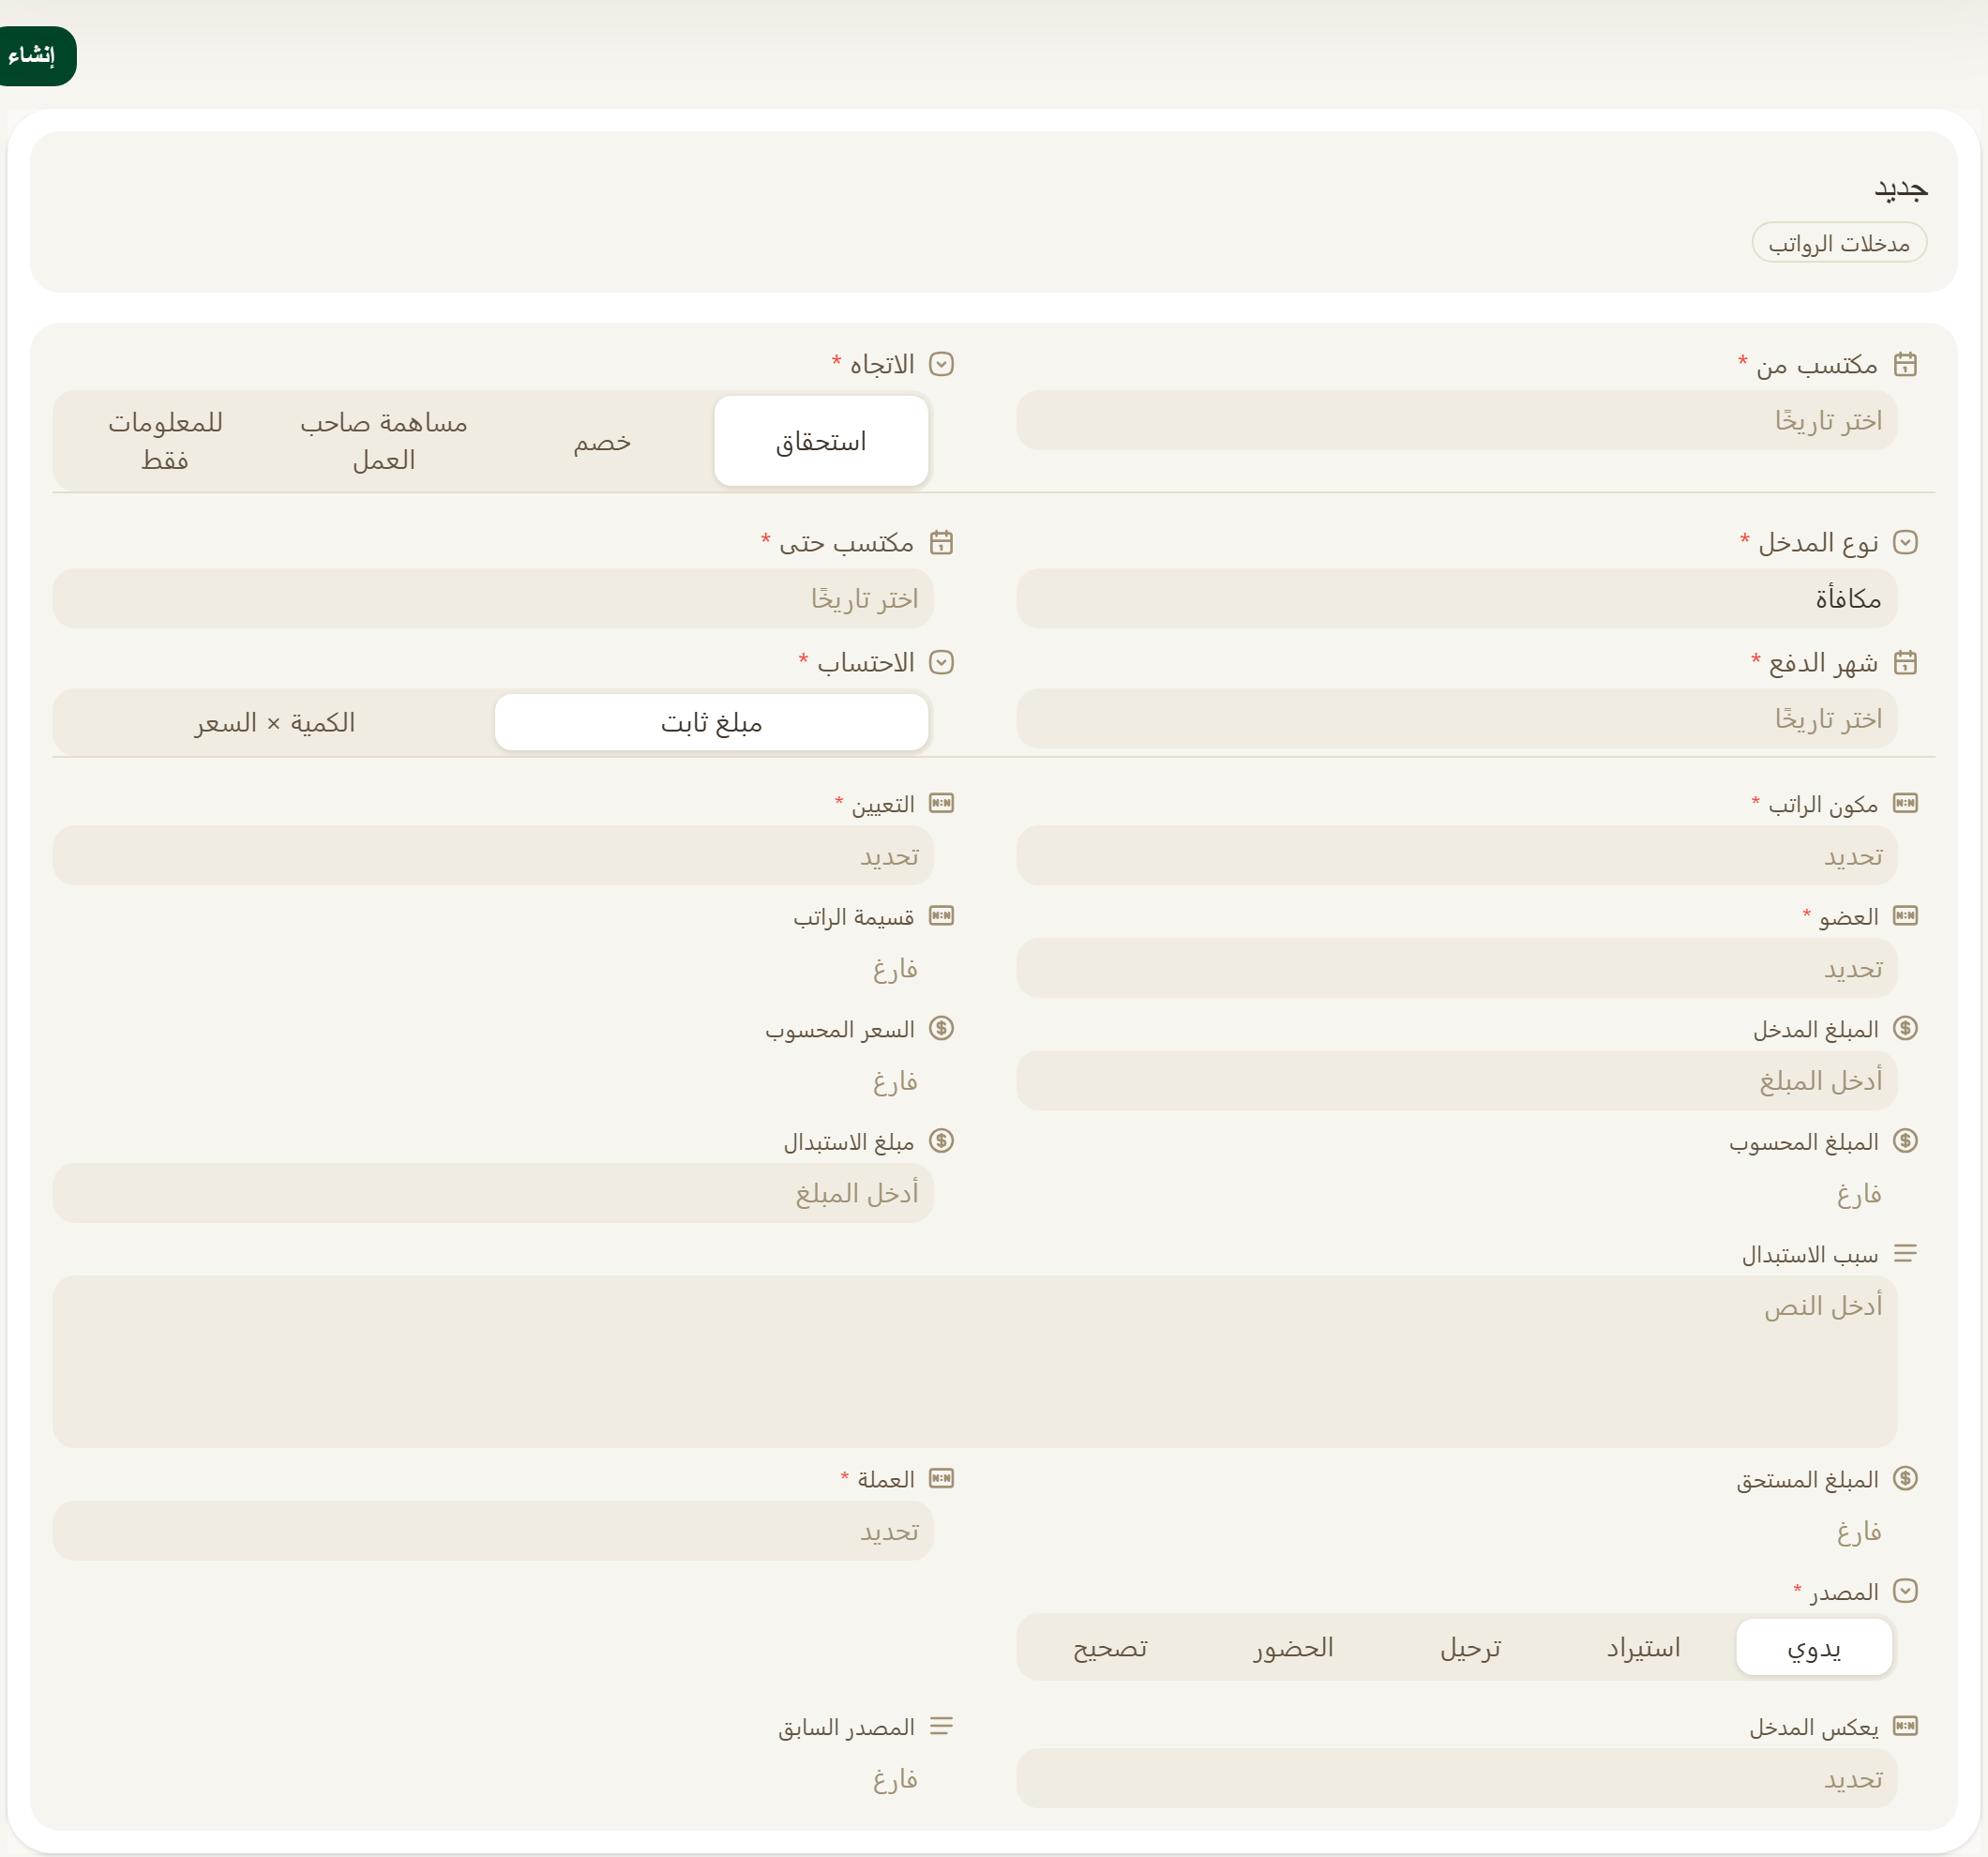
\includegraphics[width=0.95\linewidth]{figures/screens/ch03-payroll-input-fields.png}
\caption{Payroll input: complete * fields — unsaved Arabic form}
\label{fig:hr-payroll-input-screen}
\end{figure}

\textbf{Check:} amount and calculation method are correct. Preview is not payment.

\section{Slip, then payroll}

Review Sarah’s slip first. Use your organization’s approved pay and currency.

\begin{figure}[H]
\centering
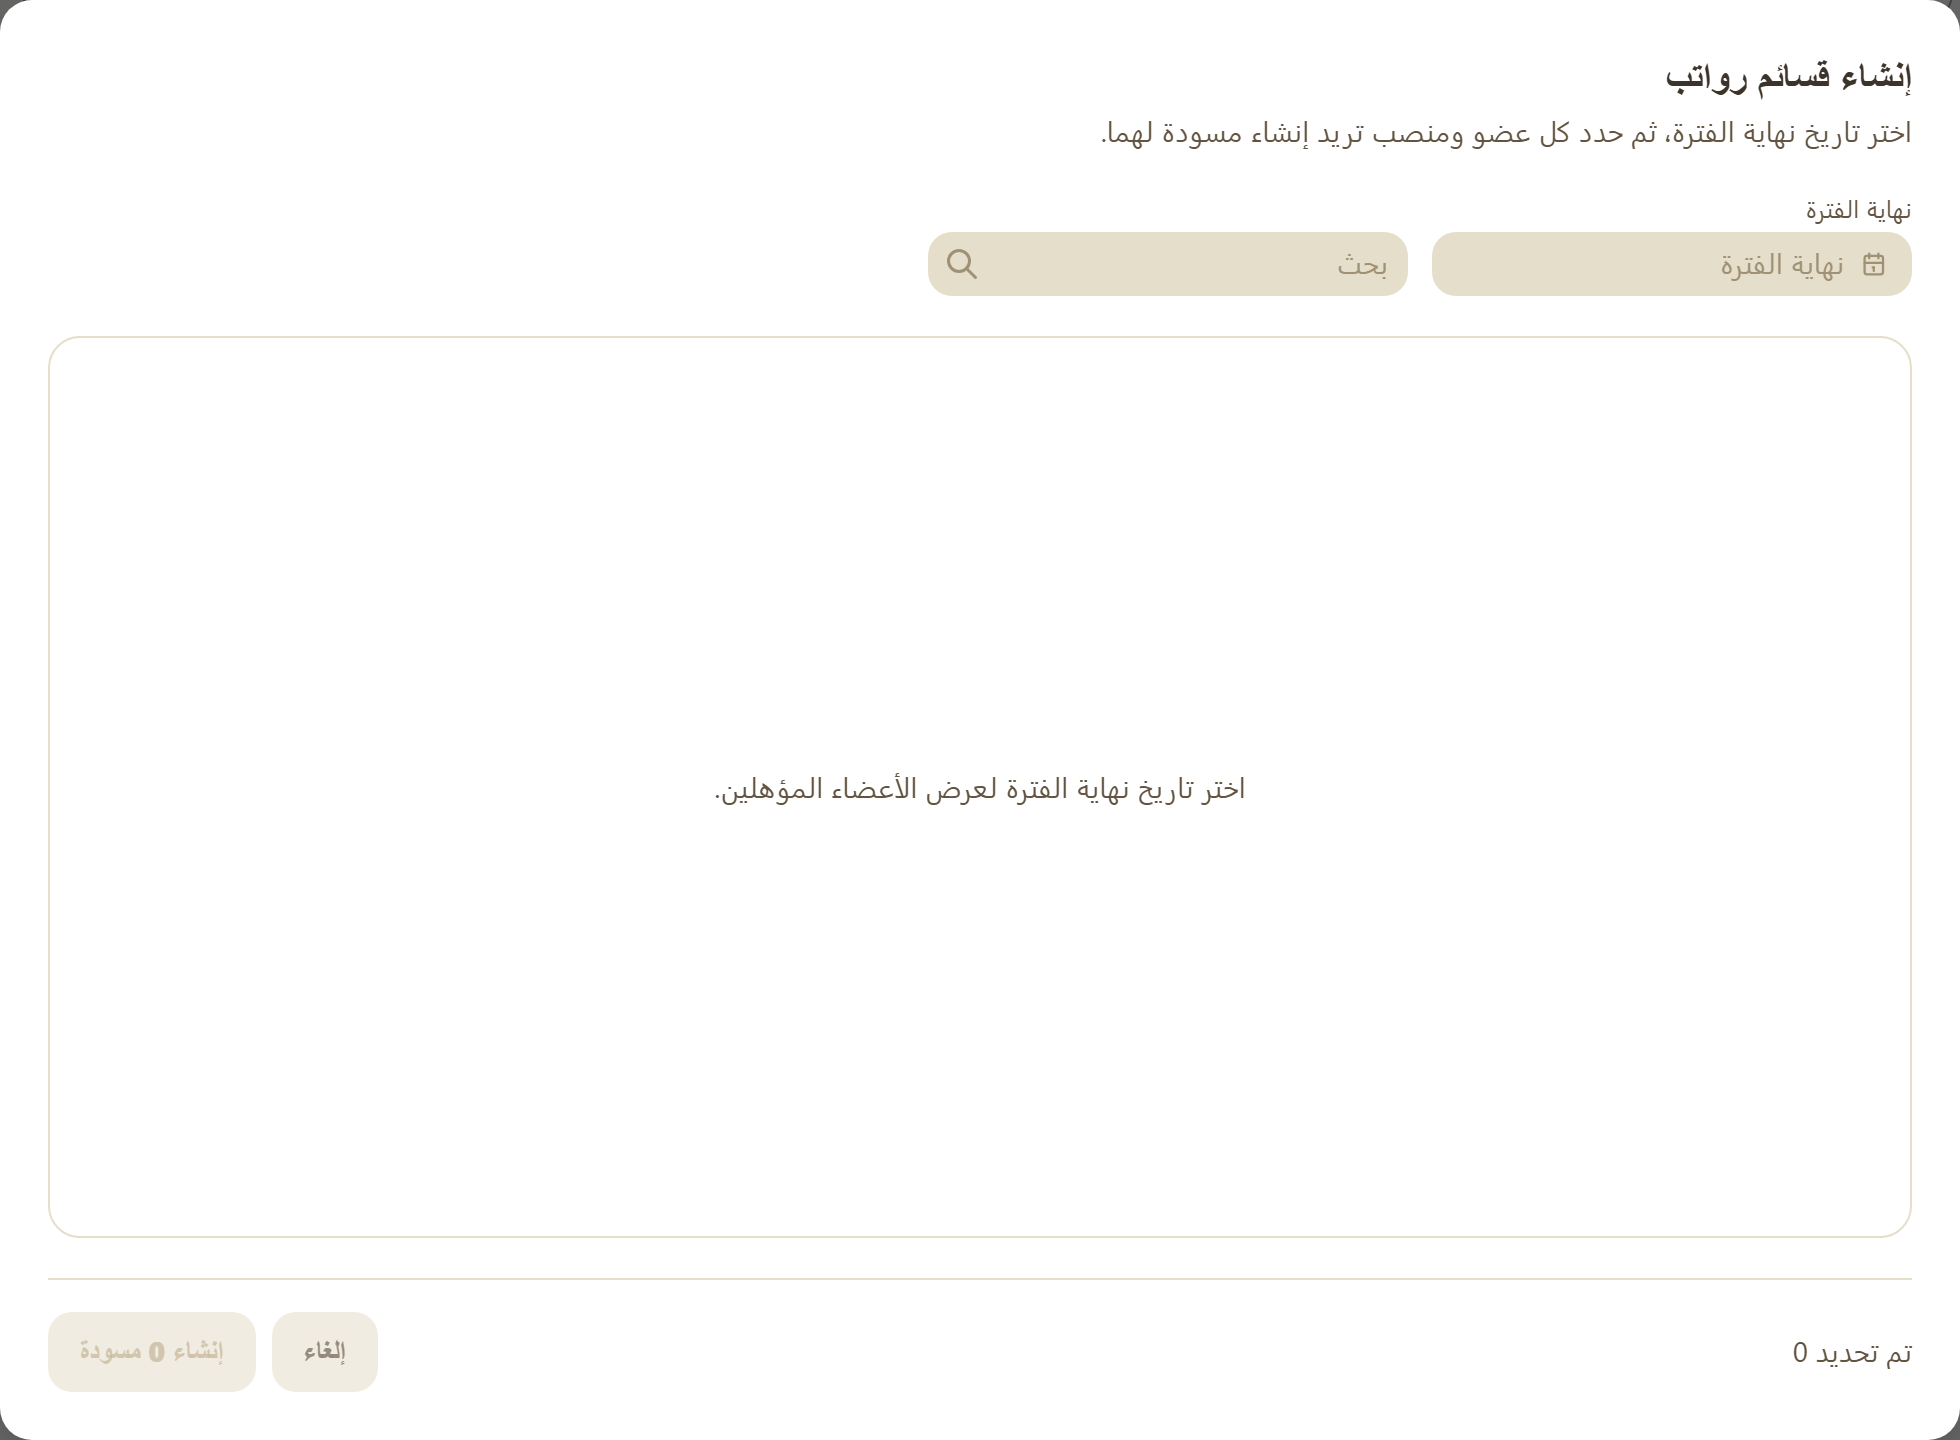
\includegraphics[width=0.95\linewidth]{figures/screens/ch03-create-slips-clear.png}
\caption{Choose Period end to list eligible employees (Arabic interface)}
\label{fig:hr-create-slips-screen}
\end{figure}

\textbf{Salary slip:}

\begin{enumerate}
  \item HR / Payment / Salary Slips / “Create salary slips”.
  \item Choose “Period end”, then Sarah’s row and position. Check “Period start”; the first slip defaults to assignment start and can be changed.
  \item Create drafts using the button showing the selected count; open her slip. If a draft exists, review it instead of duplicating.
  \item Choose “Calculate”. Check period, earnings, deductions and net pay. Use “Recalculate” after changing inputs.
  \item When items are correct, choose “Approve” as permitted. Read and confirm the prompt; check the list status.
\end{enumerate}

\textbf{Payroll:}

\begin{enumerate}
  \item Payment / Payrolls / “Generate payroll”.
  \item Set month, year, filters and employees; payroll uses approved slips in range.
  \item Choose “Generate”. Resolve conflicts with existing payroll. Open the result; check people, period, total and status.
\end{enumerate}

\textbf{Check:} trace each amount to its slip and items. If someone is missing, check period, filters, assignment and slip status.

\begin{rcwarn}[Calculation is not payment]
Check payment status and records under your organization’s procedure. Creating payroll does not prove receipt of money.
\end{rcwarn}

\section{Check and fix}
\label{sec:hr-check}

\begin{rcchecklist}[A small trial before rolling out the setup]
\begin{checklist}
  \item Sarah's member record is linked to her position by an assignment for the right period.
  \item Shift HZN-S-01 shows the required days, times and time zone.
  \item The net duration of the example shift is 07:30, and the break is inside working time.
  \item The right shift appears in the position and the assignment; any value overriding the inherited one was reviewed.
  \item An actual attendance day was reviewed; opening the attendance list was not enough.
  \item Leaves and corrections belong to the intended employee and date.
  \item If payroll was used: the items, currency and total were reviewed before approval and payment.
\end{checklist}
\end{rcchecklist}

\begin{table}[H]
\centering
\caption{Common mistakes and how to fix them}
\label{tab:hr-errors}
\rcZebra
\begin{tabularx}{\linewidth}{R{4.2cm} Y}
\rcHeaderRow
\thh{Problem} & \thh{What do you check?}\\
The shift does not save & The name, code and working days, then overlapping periods or a break outside working time.\\
The shift duration is less than expected & The breaks; they are subtracted from the total of the periods in regular and split shifts.\\
An employee is on a different shift & The assignment and the position, the unit's priority over the location, and the override option.\\
A shift cannot be deleted & It may be used in other records; check its links first.\\
An employee does not appear in the payroll & The month, the filters, the assignment and the approved pay, and any conflict with an existing payroll.\\
A leave does not give the expected result & Its type, payment method, date and duration, then the pay details for the period.\\
\end{tabularx}
\end{table}

\section{Links to other apps}

Tasks and projects use people and jobs. A leave request does not replace its leave record. For project costs, review payroll allocations; do not assume one salary belongs to one project.

